\begin{figure}[b]
\sidecaption
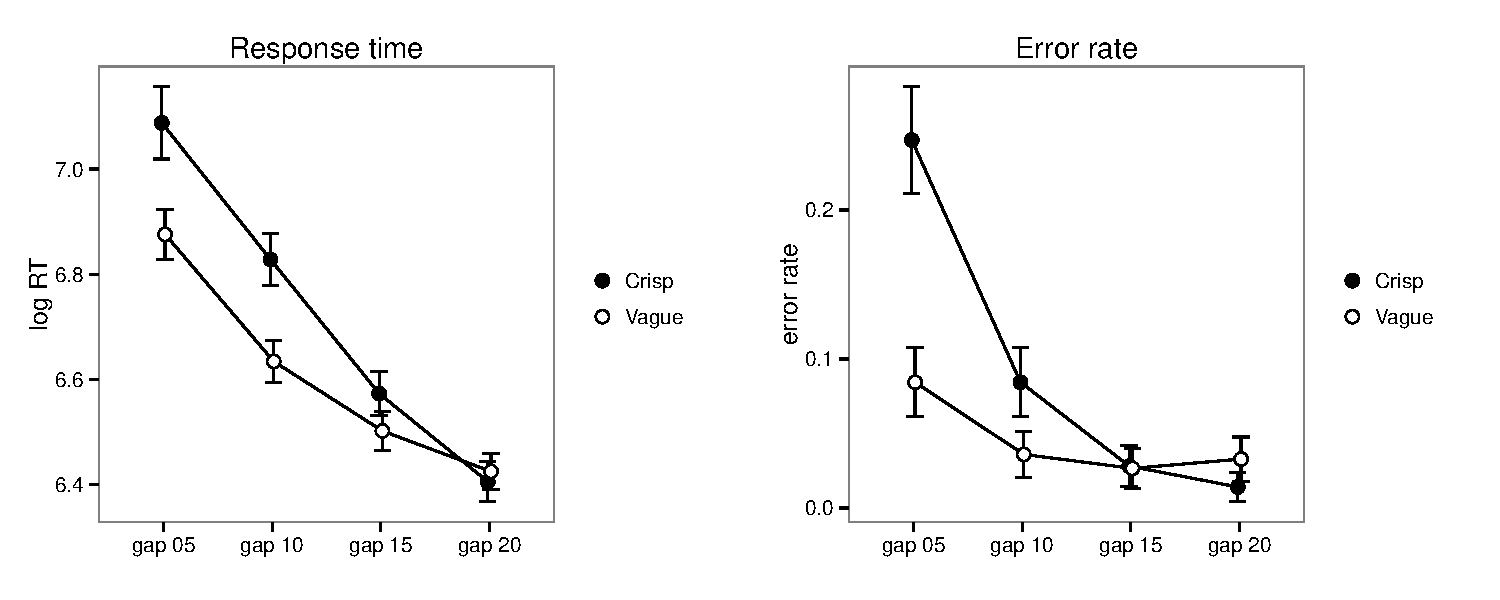
\includegraphics[scale=.5]{images/resultse1}
\caption{Experiment 1 resultsIf the width of the figure is less than 7.8 cm use the \texttt{sidecapion} command to flush the caption on the left side of the page. If the figure is positioned at the top of the page, align the sidecaption with the top of the figure -- to achieve this you simply need to use the optional argument \texttt{[t]} with the \texttt{sidecaption} command}
\label{resultse1}
\end{figure}


\begin{table}
\caption{Table of instructions for the pair (5,25). Experiment 1}
\label{instructionse1} 
\begin{tabular}{| l | l |}
\hline\noalign{\smallskip}
vagueness&example\\
\noalign{\smallskip}\svhline\noalign{\smallskip}
crisp 	& 	Choose the square with 5 dots \\
vague	&	Choose the square with few dots\\
\noalign{\smallskip}\hline\noalign{\smallskip}
\end{tabular}
$^a$ Table foot note (with superscript)\\
\end{table}


\begin{table}
\caption{}
\label{} 
\begin{tabular}{}
\hline\noalign{\smallskip}

\noalign{\smallskip}\svhline\noalign{\smallskip}

\noalign{\smallskip}\hline\noalign{\smallskip}
\end{tabular}
$^a$ Table foot note (with superscript)\\
\end{table}



\begin{theorem}
Theorem text goes here.
\end{theorem}
%
% or
%
\begin{definition}
Definition text goes here.
\end{definition}

\begin{proof}
%\smartqed
Proof text goes here.
\qed
\end{proof}

\paragraph{Paragraph Heading} %
Instead of simply listing headings of different levels we recommend to let every heading be followed by at least a short passage of text. Furtheron please use the \LaTeX\ automatism for all your cross-references and citations as has already been described in Sect.~\ref{sec:2}.

Note that the first line of text that follows a heading is not indented, whereas the first lines of all subsequent paragraphs are.
%
% For built-in environments use
%
\begin{theorem}
Theorem text goes here.
\end{theorem}
%
\begin{definition}
Definition text goes here.
\end{definition}
%
\begin{proof}
\smartqed
Proof text goes here.
\qed
\end{proof}
%

 Problems or Exercises should be sorted chapterwise
\section*{Problems}
\addcontentsline{toc}{section}{Problems}

 Use the following environment.
 Don't forget to label each problem;
% the label is needed for the solutions' environment
\begin{prob}
\label{prob1}
A given problem or Excercise is described here. The
problem is described here. The problem is described here.
\end{prob}

\begin{prob}
\label{prob2}
\textbf{Problem Heading}\\
(a) The first part of the problem is described here.\\
(b) The second part of the problem is described here.
\end{prob}



\begin{equation}
a \times b = c
\end{equation}




